\documentclass{ximera}

%\usepackage{todonotes}

\newcommand{\todo}{}

\usepackage{tkz-euclide}
\tikzset{>=stealth} %% cool arrow head
\tikzset{shorten <>/.style={ shorten >=#1, shorten <=#1 } } %% allows shorter vectors

\usepackage{tkz-tab}  %% sign charts
\usetikzlibrary{decorations.pathreplacing} 

\usetikzlibrary{backgrounds} %% for boxes around graphs
\usetikzlibrary{shapes,positioning}  %% Clouds and stars
\usetikzlibrary{matrix} %% for matrix
\usepgfplotslibrary{polar} %% for polar plots
\usetkzobj{all}
\usepackage[makeroom]{cancel} %% for strike outs
%\usepackage{mathtools} %% for pretty underbrace % Breaks Ximera
\usepackage{multicol}

\usepackage{polynom}



\usepackage[many]{tcolorbox}  %% for titled boxes
\newtcolorbox{xbox}[1]{%
    tikznode boxed title,
    enhanced,
    arc=0mm,
    interior style={white},
    attach boxed title to top center= {yshift=-\tcboxedtitleheight/2},
    fonttitle=\bfseries,
    colbacktitle=white,coltitle=black,
    boxed title style={size=normal,colframe=white,boxrule=0pt},
    title={#1}}


\usepackage{array}
\setlength{\extrarowheight}{+.1cm}   
\newdimen\digitwidth
\settowidth\digitwidth{9}
\def\divrule#1#2{
\noalign{\moveright#1\digitwidth
\vbox{\hrule width#2\digitwidth}}}





\newcommand{\RR}{\mathbb R}
\newcommand{\R}{\mathbb R}
\newcommand{\N}{\mathbb N}
\newcommand{\Z}{\mathbb Z}

%\renewcommand{\d}{\,d\!}
\renewcommand{\d}{\mathop{}\!d}
\newcommand{\dd}[2][]{\frac{\d #1}{\d #2}}
\newcommand{\pp}[2][]{\frac{\partial #1}{\partial #2}}
\renewcommand{\l}{\ell}
\newcommand{\ddx}{\frac{d}{\d x}}
\newcommand{\ddt}{\frac{d}{\d t}}

\newcommand{\zeroOverZero}{\ensuremath{\boldsymbol{\tfrac{0}{0}}}}
\newcommand{\inftyOverInfty}{\ensuremath{\boldsymbol{\tfrac{\infty}{\infty}}}}
\newcommand{\zeroOverInfty}{\ensuremath{\boldsymbol{\tfrac{0}{\infty}}}}
\newcommand{\zeroTimesInfty}{\ensuremath{\small\boldsymbol{0\cdot \infty}}}
\newcommand{\inftyMinusInfty}{\ensuremath{\small\boldsymbol{\infty - \infty}}}
\newcommand{\oneToInfty}{\ensuremath{\boldsymbol{1^\infty}}}
\newcommand{\zeroToZero}{\ensuremath{\boldsymbol{0^0}}}
\newcommand{\inftyToZero}{\ensuremath{\boldsymbol{\infty^0}}}



\newcommand{\numOverZero}{\ensuremath{\boldsymbol{\tfrac{\#}{0}}}}
\newcommand{\dfn}{\textbf}
%\newcommand{\unit}{\,\mathrm}
\newcommand{\unit}{\mathop{}\!\mathrm}
\newcommand{\eval}[1]{\bigg[ #1 \bigg]}
\newcommand{\seq}[1]{\left( #1 \right)}
\renewcommand{\epsilon}{\varepsilon}
\renewcommand{\iff}{\Leftrightarrow}

\DeclareMathOperator{\arccot}{arccot}
\DeclareMathOperator{\arcsec}{arcsec}
\DeclareMathOperator{\arccsc}{arccsc}
\DeclareMathOperator{\si}{Si}
\DeclareMathOperator{\proj}{proj}
\DeclareMathOperator{\scal}{scal}


\newcommand{\tightoverset}[2]{% for arrow vec
  \mathop{#2}\limits^{\vbox to -.5ex{\kern-0.75ex\hbox{$#1$}\vss}}}
\newcommand{\arrowvec}[1]{\tightoverset{\scriptstyle\rightharpoonup}{#1}}
\renewcommand{\vec}{\mathbf}
\newcommand{\veci}{\vec{i}}
\newcommand{\vecj}{\vec{j}}
\newcommand{\veck}{\vec{k}}
\newcommand{\vecl}{\boldsymbol{\l}}

\newcommand{\dotp}{\bullet}
\newcommand{\cross}{\boldsymbol\times}
\newcommand{\grad}{\boldsymbol\nabla}
\newcommand{\divergence}{\grad\dotp}
\newcommand{\curl}{\grad\cross}
%\DeclareMathOperator{\divergence}{divergence}
%\DeclareMathOperator{\curl}[1]{\grad\cross #1}


\colorlet{textColor}{black} 
\colorlet{background}{white}
\colorlet{penColor}{blue!50!black} % Color of a curve in a plot
\colorlet{penColor2}{red!50!black}% Color of a curve in a plot
\colorlet{penColor3}{red!50!blue} % Color of a curve in a plot
\colorlet{penColor4}{green!50!black} % Color of a curve in a plot
\colorlet{penColor5}{orange!80!black} % Color of a curve in a plot
\colorlet{fill1}{penColor!20} % Color of fill in a plot
\colorlet{fill2}{penColor2!20} % Color of fill in a plot
\colorlet{fillp}{fill1} % Color of positive area
\colorlet{filln}{penColor2!20} % Color of negative area
\colorlet{fill3}{penColor3!20} % Fill
\colorlet{fill4}{penColor4!20} % Fill
\colorlet{fill5}{penColor5!20} % Fill
\colorlet{gridColor}{gray!50} % Color of grid in a plot

\newcommand{\surfaceColor}{violet}
\newcommand{\surfaceColorTwo}{redyellow}
\newcommand{\sliceColor}{greenyellow}




\pgfmathdeclarefunction{gauss}{2}{% gives gaussian
  \pgfmathparse{1/(#2*sqrt(2*pi))*exp(-((x-#1)^2)/(2*#2^2))}%
}


%%%%%%%%%%%%%
%% Vectors
%%%%%%%%%%%%%

%% Simple horiz vectors
\renewcommand{\vector}[1]{\left\langle #1\right\rangle}


%% %% Complex Horiz Vectors with angle brackets
%% \makeatletter
%% \renewcommand{\vector}[2][ , ]{\left\langle%
%%   \def\nextitem{\def\nextitem{#1}}%
%%   \@for \el:=#2\do{\nextitem\el}\right\rangle%
%% }
%% \makeatother

%% %% Vertical Vectors
%% \def\vector#1{\begin{bmatrix}\vecListA#1,,\end{bmatrix}}
%% \def\vecListA#1,{\if,#1,\else #1\cr \expandafter \vecListA \fi}

%%%%%%%%%%%%%
%% End of vectors
%%%%%%%%%%%%%

%\newcommand{\fullwidth}{}
%\newcommand{\normalwidth}{}



%% makes a snazzy t-chart for evaluating functions
%\newenvironment{tchart}{\rowcolors{2}{}{background!90!textColor}\array}{\endarray}

%%This is to help with formatting on future title pages.
\newenvironment{sectionOutcomes}{}{} 



%% Flowchart stuff
%\tikzstyle{startstop} = [rectangle, rounded corners, minimum width=3cm, minimum height=1cm,text centered, draw=black]
%\tikzstyle{question} = [rectangle, minimum width=3cm, minimum height=1cm, text centered, draw=black]
%\tikzstyle{decision} = [trapezium, trapezium left angle=70, trapezium right angle=110, minimum width=3cm, minimum height=1cm, text centered, draw=black]
%\tikzstyle{question} = [rectangle, rounded corners, minimum width=3cm, minimum height=1cm,text centered, draw=black]
%\tikzstyle{process} = [rectangle, minimum width=3cm, minimum height=1cm, text centered, draw=black]
%\tikzstyle{decision} = [trapezium, trapezium left angle=70, trapezium right angle=110, minimum width=3cm, minimum height=1cm, text centered, draw=black]


\title[Dig-In:]{Relating velocity and position}


\begin{document}
\begin{abstract}
\end{abstract}
\maketitle

A central theme of this course has been that we can often gain a
better understanding of a function by looking at its derivative, and
then working backwards.  This has been our approach to max/min
problems, curve sketching, linear approximation, and so on.  So
antiderivatives have really been important to us all along.

We have a graphical interpretation of the derivative as the slope of a
tangent line at a point.  We have not yet found a graphical
interpretation of the antiderivative.

  \begin{question}
   Let $f$ be the constant function $4$. Let $F$ be any antiderivative
   of $f$.  Then $F(5)-F(2) = \answer{12}$.
   \begin{hint}
    This is just a fancy way of saying that $f$ is a line of slope
    $4$, and we are looking for the rise corresponding to a run of
    $5-2= 3$
   \end{hint}
   \begin{hint}
    $F(5) - F(2) = 4(5-2) = 12$
   \end{hint}
  \end{question}
  
  \begin{question}
    The area of the region bounded by the graph of $f$, the horizontal
    axis, and the vertical lines $x=2$ and $x=5$ is $\answer{12}$.
    
    \begin{hint}
      \begin{image}
  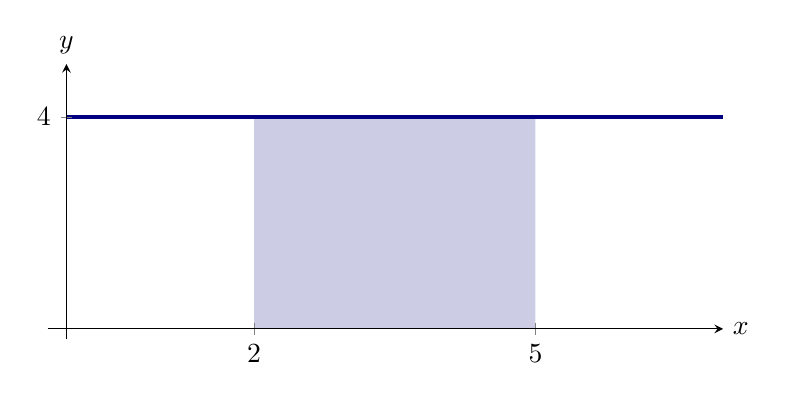
\begin{tikzpicture}[
      declare function = {f(\x) = 4;} ]
	\begin{axis}[
            domain=-.2:7, xmin =-.2,xmax=7,ymax=5,ymin=-.2,
            width=4in,
            height=2in,
            xtick={2,5}, 
	   ytick={4},
            xticklabels={$2$,$5$},
            yticklabels={$4$},
            axis lines=center, xlabel=$x$, ylabel=$y$,
            every axis y label/.style={at=(current axis.above origin),anchor=south},
            every axis x label/.style={at=(current axis.right of origin),anchor=west},
            axis on top,
          ]
          \addplot [draw=none,fill=fillp,domain=2:5, smooth] {f(x)} \closedcycle;
          \addplot [very thick,penColor, smooth, domain=0:7] {f(x)};
        \end{axis}
\end{tikzpicture}
\end{image}
    \end{hint}
    \begin{hint}
      This is a rectangle with height $4$ and width $3$, so the area is $12$
    \end{hint}
  \end{question}


The fact that these two answers are the same is the germ of one of the
most ``fundamental'' ideas in all of calculus. However, before we can
step ahead, we might first look back to our even younger days of being mathemaitcians.

%\begin{idea}[Two models of multiplication]
  There are two basic models of multiplication: A ``rate times time''
  perpective and an ``area'' perspective.  For instance, we could
  interpret
  \[
  3\times 4
  \]
  as an answer to the question:
  \begin{center}
    ``If I am going $3 \textrm{mph}$ for $4$ hours, how far have I
    traveled?''
  \end{center}
  or as the answer to the question
  \begin{center}
    ``What is the area of a rectangle with length $3$ and width $4$?''
  \end{center}
    %\end{idea}

It is this dual interperating that will allow us to begin to
understand a geometric meaning of the antiderivative.

Let $v(t)$ be the velocity of some object at time $t$.
\begin{image}
  \begin{tikzpicture}[
      declare function = {f(\x) = cos((\x-1.1)*360/6.28);} ]
	\begin{axis}[
            domain=-.2:4, xmin =-.2,xmax=4,ymax=1.1,ymin=-1.1,
            width=4in,
            height=2in,
            xtick={1,3}, 
            xticklabels={$1$,$3$},
            ytick style={draw=none},
            yticklabels={},
            axis lines=center, xlabel=$t$, ylabel=$y$,
            every axis y label/.style={at=(current axis.above origin),anchor=south},
            every axis x label/.style={at=(current axis.right of origin),anchor=west},
            axis on top,
          ]

          \addplot [very thick,penColor, smooth] {f(x)};
          \node at (axis cs:3.5,4.5) [anchor=west] {$f$};  


        \end{axis}
\end{tikzpicture}
\end{image}
and let $F$ be an antiderivative of $f$.  Suppose we want to approximate $F(3)
- F(1)$.  Let's get an approximation using $4$ subintervals.
  
  \begin{align*}F(3) - F(1) &= (F(3) - F(2.5))+(F(2.5) - F(2))+(F(2) - F(1.5))+(F(1.5) - F(1))\\
  &\approx F'(3)\frac{1}{2}+F'(2.5)\frac{1}{2}+F'(2)\frac{1}{2}+F'(1.5)\frac{1}{2}\\
  &=f(3)\frac{1}{2}+f(2.5)\frac{1}{2}+f(2)\frac{1}{2}+f(1.5)\frac{1}{2}
  \end{align*}
  
  We can visualize this as the sum of the areas of $4$ rectangles.  Note that while the first $3$ terms are positive, the last is negative because $f(3)<0$.  We should think of these rectangles as having \textbf{signed area}, where the area is negative when it lives below the $x$-axis. 

\begin{image}
  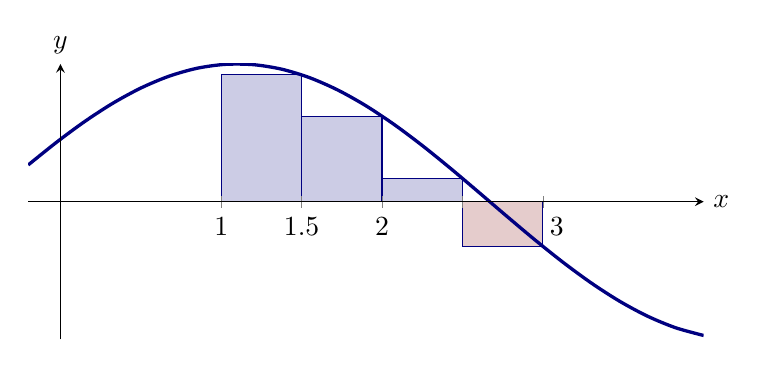
\begin{tikzpicture}[
      declare function = {f(\x) = cos((\x-1.1)*360/6.28);} ]
	\begin{axis}[
            domain=-.2:4, xmin =-.2,xmax=4,ymax=1,ymin=-1,
            width=4in,
            height=2in,
            xtick={1,1.5,2,2.5,3}, 
            xticklabels={$1$,$1.5$,$2$, , $ \hphantom{22}3$},
            ytick style={draw=none},
            yticklabels={},
            axis lines=center, xlabel=$x$, ylabel=$y$,
            every axis y label/.style={at=(current axis.above origin),anchor=south},
            every axis x label/.style={at=(current axis.right of origin),anchor=west},
            axis on top,
          ]


\foreach \rectnumber in {1,2,3}
               {
                 \addplot [draw=penColor,fill=fillp] plot coordinates
                          {({1+(\rectnumber - 1) * 0.5},{f(1+\rectnumber * 0.5)})
                            ({1+(\rectnumber) * 0.5},{f(1+\rectnumber * 0.5) })} \closedcycle;

          
               };

 \addplot [draw=penColor,fill=filln] plot coordinates
                          {({1+(4 - 1) * 0.5},{f(1+4 * 0.5)})
                            ({1+(4) * 0.5},{f(1+4 * 0.5) })} \closedcycle;
	
         \addplot [very thick,penColor, smooth] {f(x)};
          \node at (axis cs:3.5,4.5) [anchor=west] {$f$};  
        \end{axis}
\end{tikzpicture}
\end{image}
  
By approximating $f$ by a piecewise constant function, we are approximating $F$ by a piecewise linear function:

\begin{image}
  \begin{tikzpicture}[
      declare function = {f(\x) = cos((\x-1.1)*360/6.28);} ]
	\begin{axis}[
            domain=-.2:4, xmin =-.2,xmax=4,ymax=0,ymin=1,
            width=4in,
            height=2in,
            xtick={1,1.5,2,2.5,3}, 
            xticklabels={$1$,$1.5$,$2$, $2.5$, $3$},
            ytick style={draw=none},
            yticklabels={},
            axis lines=center, xlabel=$x$, ylabel=$y$,
            every axis y label/.style={at=(current axis.above origin),anchor=south},
            every axis x label/.style={at=(current axis.right of origin),anchor=west},
            axis on top,
          ]

          \addplot [very thick,penColor2, smooth, domain=1:1.5] {f(1.5)*(x-1)};
          \addplot [very thick,penColor2, smooth, domain=1.5:2] {f(2)*(x-1.5)+f(1.5)*0.5};
          \addplot [very thick,penColor2, smooth, domain=2:2.5] {f(2.5)*(x-2)+f(2)*0.5+f(1.5)*0.5};
          \addplot [very thick,penColor2, smooth, domain=2.5:3] {f(3)*(x-2.5)+f(2.5)*(0.5)+f(2)*0.5+f(1.5)*0.5};

  \addplot [draw=penColor] plot coordinates {(1,0) (1.5,0) (1.5, {f(1.5)*(0.5)}) (2, {f(1.5)*(0.5)}) (2, {f(2)*0.5+f(1.5)*0.5}) (2.5, {f(2)*0.5+f(1.5)*0.5}) (2.5, {f(2.5)*(0.5)+f(2)*0.5+f(1.5)*0.5}) (3, {f(2.5)*(0.5)+f(2)*0.5+f(1.5)*0.5})  (3, { f(3)*0.5+f(2.5)*(0.5)+f(2)*0.5+f(1.5)*0.5})};

          \node at (axis cs:3.1,10) [anchor=west] {$F$};  
        \end{axis}
\end{tikzpicture}
\end{image}


  
  On the one hand, we can interpret each $F'(x)\Delta x$ as an approximation in the change in the height of $F$ over the subinterval.  On the other hand, since $F' =f$, we can think of $F'(x)\Delta x = f(x)\Delta x$ as the area of a rectangle based on the subinterval, and with hieght $f(x)$.  So the total change in $F$ over $[1,3]$ can be reinterpreted as the sum of the signed areas of the rectangles under $f$.
  
If we make our subintervals smaller, the repeated linear approximation should get more precise, and the sum of the areas of the rectangles gets closer to the area under the curve:

\begin{image}
  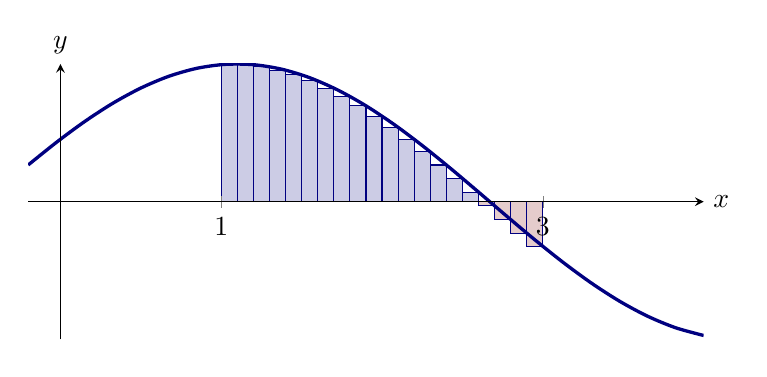
\begin{tikzpicture}[
      declare function = {f(\x) = cos((\x-1.1)*360/6.28);} ]
	\begin{axis}[
            domain=-.2:4, xmin =-.2,xmax=4,ymax=1,ymin=-1,
            width=4in,
            height=2in,
            xtick={1,3}, 
            xticklabels={$1$,$3$},
            ytick style={draw=none},
            yticklabels={},
            axis lines=center, xlabel=$x$, ylabel=$y$,
            every axis y label/.style={at=(current axis.above origin),anchor=south},
            every axis x label/.style={at=(current axis.right of origin),anchor=west},
            axis on top,
          ]
        
\foreach \rectnumber in {1,2,...,16}
               {
                 \addplot [draw=penColor,fill=fillp] plot coordinates
                          {({1+(\rectnumber - 1) * 0.1},{f(1+\rectnumber * 0.1)})
                            ({1+(\rectnumber) * 0.1},{f(1+\rectnumber * 0.1) })} \closedcycle;

            
               };

\foreach \rectnumber in {17,18,19,20}
               {
                 \addplot [draw=penColor,fill=filln] plot coordinates
                          {({1+(\rectnumber - 1) * 0.1},{f(1+\rectnumber * 0.1)})
                            ({1+(\rectnumber) * 0.1},{f(1+\rectnumber * 0.1) })} \closedcycle;

            
               };
          \addplot [very thick,penColor, smooth] {f(x)};
          \node at (axis cs:3.5,4.5) [anchor=west] {$f$};  
        \end{axis}
\end{tikzpicture}
\end{image}

So it is reasonable to think that $F(3) - F(1)$ should be exactly equal to the \textbf{signed area} under the graph of $f$.

%This definition needs work...
\begin{definition}
To find the \textbf{signed area} of $f$ from $x=a$ to $x=b$, sum the positive area of all those regions lying above the $x$ axis, and subtract the area of all those regions lying below the $x$-axis.
\end{definition}

\begin{observation}
	Our investigations above lead us to suspect that, if $F' = f$, then $F(b) - F(a)$ should be equal to the signed area under $f$ from $a$ to $b$.  
\end{observation}

\begin{question}
Assume a particle is accelerating at a constant rate of $3 \frac{m}{s^2}$, and starts at velocity of $-3 \frac{m}{s}$ and travels for $5$ seconds.  Draw a graph of the velocity as a function of time, and use the ideas in this section to compute the displacement of the particle over its journey.

\begin{hint}
	The graph of velocity versus time looks like this:

\begin{image}
  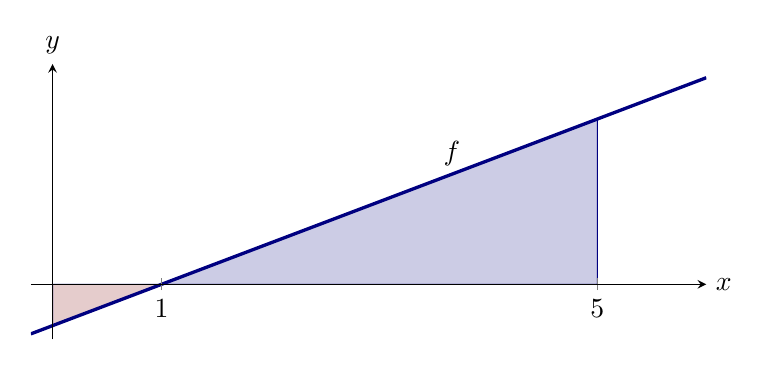
\begin{tikzpicture}[
      declare function = {f(\x) = 3*\x-3;} ]
	\begin{axis}[
            domain=-.2:6, xmin =-.2,xmax=6,ymax=16,ymin=-4,
            width=4in,
            height=2in,
            xtick={1,5}, 
            xticklabels={$1$,$5$},
            ytick style={draw=none},
            yticklabels={},
            axis lines=center, xlabel=$x$, ylabel=$y$,
            every axis y label/.style={at=(current axis.above origin),anchor=south},
            every axis x label/.style={at=(current axis.right of origin),anchor=west},
            axis on top,
          ]
	
	\addplot [draw=penColor,fill=filln] plot coordinates
                          {(0,-3) (1,0)} \closedcycle;

	\addplot [draw=penColor,fill=fillp] plot coordinates
                          {(1,0) (5,12)} \closedcycle;

          \addplot [very thick,penColor, smooth] {f(x)};
          \node at (axis cs:3.5,9.5) [anchor=west] {$f$};  
        \end{axis}

\end{tikzpicture}
\end{image}
	
\end{hint}

\begin{hint}
	Since velocity is the derivative of position with respect to time, then by our discussion above the change in position should be the signed area under the velocity curve.  You can compute this as the difference in the areas of two triangles.
\end{hint}

\begin{hint}
	The blue triangle has area $\frac{1}{2}(5-1)(12) = 24$, and the red triangle has area $\frac{1}{2}(1)(3) = \frac{3}{2}$.  So the net area is $24-\frac{3}{2} = \frac{45}{2}$.  This is the displacement of the particle!
\end{hint}

The displacement of the particle is $\answer{\frac{45}{2}}$ meters in the positive direction.

\begin{feedback}
You could have also solved this problem by finding an antiderivative.  Try that method and see how it compares.  Does this geometry shed light on your understanding of constant acceleration?
\end{feedback}
\end{question}


  
\end{document}
